\tocchapter{Proiektuaren helburu dokumentua}

\section{Deskribapena}
Garatuko den aplikazioa azpititulu editore bat izango da, Mac OS X sistema eragilerako. Azpititulu berriak sortu edo sortuta daudenak editatu ahal izango ditu, formatu erabilienetan: ASS, SRT eta SUB. TXT fitxategiak ere inportatu ahal izango ditu azpitituluen sorrerarako.

\section{Helburua}
Helburu nagusia aplikazioaren garapena da, horretarako hainbat zelai ikutzen direlarik: fitxategien maneiua, audio fitxategien erabilera (audioa marrazteko eta erreproduzitzeko), karaokeen sorkuntza, etab.
Aplikazioaren atal gehienak programatu beharko dira, nahiz eta agian zenbait software edo liburutegi erabiliko diren gure aplikazioak behar duen funtzionalitate bat eskaintzen badute.
Proiektua lizentzia aske baten menpe garatuko da, \textbf{GNU GPVv2} hain zuzen ere, honako arrazoiengatik:
\begin{itemize}
\item Edonork aplikazioa mugarik gabe erabili ahal izatea.
\item Proiektua amaitzean, norbaitek jarraitu nahi badu ia arazorik gabe egin ahal izatea (lizentzia berdinarekin).
\item Aplikazioaren kalitatea hobetzea (jende gehiagok erabili/garatu).
\end{itemize}
Beste helburu bat, proiektu \textit{handi} baten garapenak suposatzen duena ulertzea eta dokumentatzea da.
Azkenik, proiektuen garapenarekin zerikusia duten tresnak erabiliko dira: bertsioen kontrol sistema (Subversion), bug-en gestio sistema, etab. Honetarako, Assembla.com webguneak dohainik eskaintzen dituen baliabideak erabiliko dira. Bertan proiekturako \textit{space} bat sortuko da eta honako zerbitzuak erabili ahal izango ditugu: foroak, wikiak, ticket-ak, Subversion bertsioen kontrol sistema bezala, fitxategiak igotzeko aukera, etab.

\section{Norainokoa}
Hauek dira egin beharrekoak:
\begin{enumerate}
\item Aplikazioaren garapena:
	\begin{itemize}
	\item Formatu desberdinekin lan egitea (ASS, SRT eta SUB).
	\item Audioa ireki ahal izatea hau marrazteko eta erreproduzitzeko.
	\item Zenbait laguntzaileren sorrera (itzulpenerako, karaokeak sortzeko, etab.).
	\end{itemize}
\item Aplikazioa sistemarekin ondo integratzea.
\item Erabiltzailearentzako erabilpen gidak sortzea, hau da, programaren funtzionalitateak dokumentatzea.
\item Instalatzeko erraza den pakete bat sortzea, erabiltzaileak programa konpilatu behar ez izateko.
\end{enumerate}

\subsection{Lanaren dekonposaketa egitura diagrama}
\begin{figure}[htb]
\begin{center}
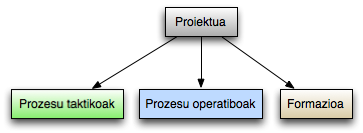
\includegraphics[width=\columnwidth, natwidth=817pt, natheight=349pt]{Pictures/Chapter3/LDE.png}
\caption{Lanaren dekonposaketa egitura diagrama}
\label{lde}
\end{center}
\end{figure}

\subsection{Azpiatazen zerrenda}
\begin{itemize}
\item \textbf{Kudeaketa:}
	\begin{itemize}
	\item K1 - Bilerak:
		\begin{itemize}
		\item K11 - Ohiko bilerak.
		\item K12 - Aurrerapen bilerak:
			\begin{itemize}
			\item K121 - Bilera burutu.
			\item K122 - Egoera txostena egin.
			\end{itemize} 
		\end{itemize}
	\item K2 - Artxiboaren kudeaketa.
	\end{itemize}
\item \textbf{Planifikazioa:}
	\begin{itemize}
	\item P1 - Proiektuaren helburu dokumentua egin.
	\item P2 - Iterazio berriaren planifikazioa.
	\end{itemize}
\item \textbf{Garapena:}
	\begin{itemize}
	\item G1 - Eskakizunen bilketa:
		\begin{itemize}
		\item G11 - Erabilpen kausen eredua egin.
		\item G12 - Domeinuaren eredua egin.
		\item G13 - Interfazearen prototipoa egin.
		\end{itemize}
	\item G2 - Analisia:
		\begin{itemize}
		\item G21 - Sistemako sekuentzia diagramak egin.
		\item G22 - Kontratuak egin.
		\end{itemize}
	\item G3 - Diseinua:
		\begin{itemize}
		\item G31 - Sekuentzia diagramak egin.
		\item G32 - Klase diagrama egin.
		\item G33 - Probak diseinatu.
		\end{itemize}
	\item G4 - Inplementazioa.
	\item G5 - Probak egin.
	\end{itemize}
\item \textbf{Dokumentazioa:}
	\begin{itemize}
	\item D1 - Eskuliburua egin.
	\item D2 - Memoria egin.
	\end{itemize}
\item \textbf{Bukatzea:}
	\begin{itemize}
	\item B1 - Defentsa:
		\begin{itemize}
		\item B11 - Edukiak aukeratu.
		\item B12 - Aurkezpena prestatu.
		\item B13 - Aurkezpena egin.
		\end{itemize}
	\end{itemize}
\item \textbf{Formazioa:}
	\begin{itemize}
	\item F1 - Aurrekarien analisia:
		\begin{itemize}
		\item F12 - Azpititulu editoreen bilaketa.
		\item F13 - Aukeratutako editoreen analisia.
		\item F14 - Konparaketa eta ondorioak.
		\end{itemize}
	\item F2 - Objective-C ikastea.
	\item F3 - Cocoa ikastea.
	\end{itemize}
\end{itemize}

\subsection{Emangarrien zerrenda}
\begin{longtable}{|p{70px}|p{250px}|p{30px}|}
\hline
\grey \textbf{Emangarria} & \grey \textbf{Deskribapena} & \grey \textbf{Ataza}\\
\hline
\endhead
\hline
\caption{\label{emangarriak}Sortuko diren emangarriak}
\endfoot
\textit{Akta} & Bilera bakoitzean tratazen diren gaien laburpena & K11\\
\hline
\textit{Egoera txostena} & Proiektuaren faseen egoera aztertzen duen dokumentua & K122\\
\hline
\textit{PHD} & Proiektua planifikatzeko hasierako unean sortutako dokumentu aldaezina & P1\\
\hline
\textit{LDE diagrama} & Ataza eta azpiataza garrantzitsuenak adierazten dituen diagrama & P1\\
\hline
\textit{Gantt diagrama} & Planifikatutako ekintzen egutegiaren adierazpide grafikoa, non ekintza bakoitzaren iraupena adierazten den & P1\\
\hline
\textit{Erabilpen kasuen eredua} & Programaren portaera adierazten duen diagrama & G11\\
\hline
\textit{Domeinuaren eredua} & Domeinuan agertzen diren objektuen atributuak eta erlazioak adierazten dituen diagrama & G12\\
\hline
\textit{Interfazearen prototipoa} & Interfazea nolakoa izango den & G13\\
\hline
\textit{Sistemako sekuentzia diagramak} & Erabilpen kasu bakoitzaren portaera adierazten duten diagramak & G21\\
\hline
\textit{Kontratuak} & Eragiketen espezifikazioa & G22\\
\hline
\textit{Sekuentzia diagramak} & Eragiketa bakoitzaren portaera adierazten duten diagramak & G31\\
\hline
\textit{Klase diagrama} & Sistemaren egitura deskribatzen duen diagrama estatikoa, non sistemako klaseak eta hauen atributu eta erlazioak agertzen diren & G32\\
\hline
\textit{Programa} & Inplementazioa amaitzean sortuko den exekutagarria & G4\\
\hline
\textit{Eskuliburua} & Programaren funtzionamendua azaltzen duen dokumentua & D1\\
\hline
\textit{Memoria} & Proiektuko lan guztia laburbiltzen duen dokumentua & D2\\
\hline
\textit{Aurkezpena} & Defentsan erabiliko diren gardenkiak & B12\\
\end{longtable}

\section{Planifikazioa}

\subsection{Denboraren estimazioa}
\begin{longtable}{|l|l|}
\hline
\grey \textbf{Ataza} & \grey \textbf{Estimazioa}\\
\hline
\endhead
\hline
\caption{\label{estimazioa}Denboraren estimazioa}
\endfoot
\bblue Kudeaketa & \bblue 30 \\
\hline
\blue Bilerak & \blue 25 \\
\hline
Ohiko bilerak & 20 \\
\hline
Aurrerapen bilerak & 5 \\
\hline
\blue Artxiboaren kudeaketa & \blue 5 \\
\hline
\bblue Planifikazioa & \bblue 10 \\
\hline
\blue PHD egin & \blue 7 \\
\hline
\blue Iterazio berriaren planifikazioa & \blue 3 \\
\hline
\bblue Garapena & \bblue 130 \\
\hline
\blue Eskakizunen bilketa & \blue 10 \\
\hline
\blue Analisia & \blue 15 \\
\hline
\blue Diseinua & \blue 25 \\
\hline
\blue Inplementazioa & \blue 55 \\
\hline
\blue Probak egin & \blue 25 \\
\hline
\bblue Dokumentazioa & \bblue 60 \\
\hline
\blue Eskuliburua egin & \blue 15 \\
\hline
\blue Memoria egin & \blue 45 \\
\hline
\bblue Bukatzea & \bblue 10 \\
\hline
\blue Defentsa & \blue 10 \\
\hline
\bblue Formazioa & \bblue 60 \\
\hline
\blue Aurrekarien analisia & \blue 10 \\
\hline
\blue Objective-C ikasi & \blue 30 \\
\hline
\blue Cocoa ikasi & \blue 20 \\
\hline
\grey \textbf{Guztira} & \grey 300 ordu \\
\end{longtable}

\subsection{Denbora plangintza: GANTT diagrama}
\ref{gantt}~Irudian agertzen da proiektuaren denbora plangintza.
\begin{figure}[htp]
\begin{center}
%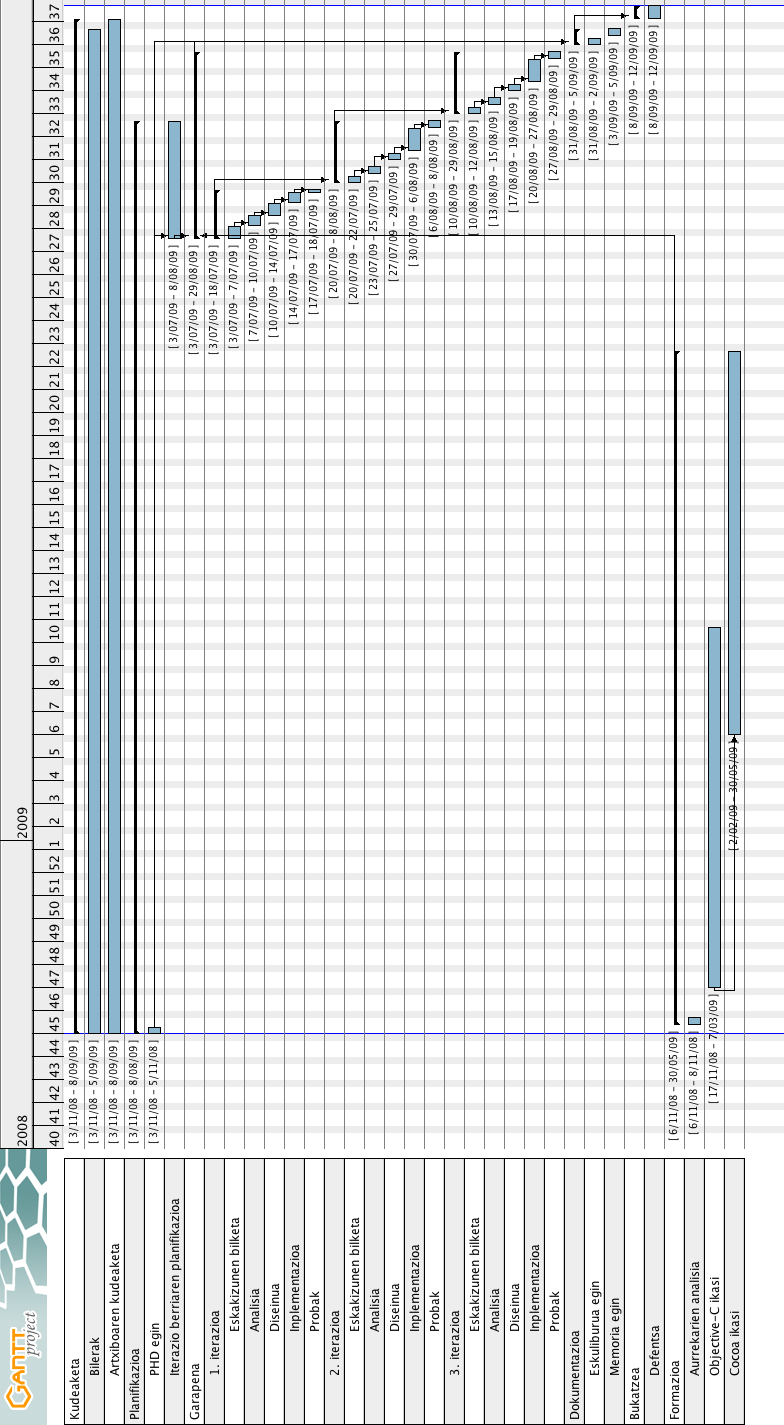
\includegraphics[width=\columnwidth, natwidth=784pt, natheight=1425pt]{Pictures/Chapter3/Gantt.png}
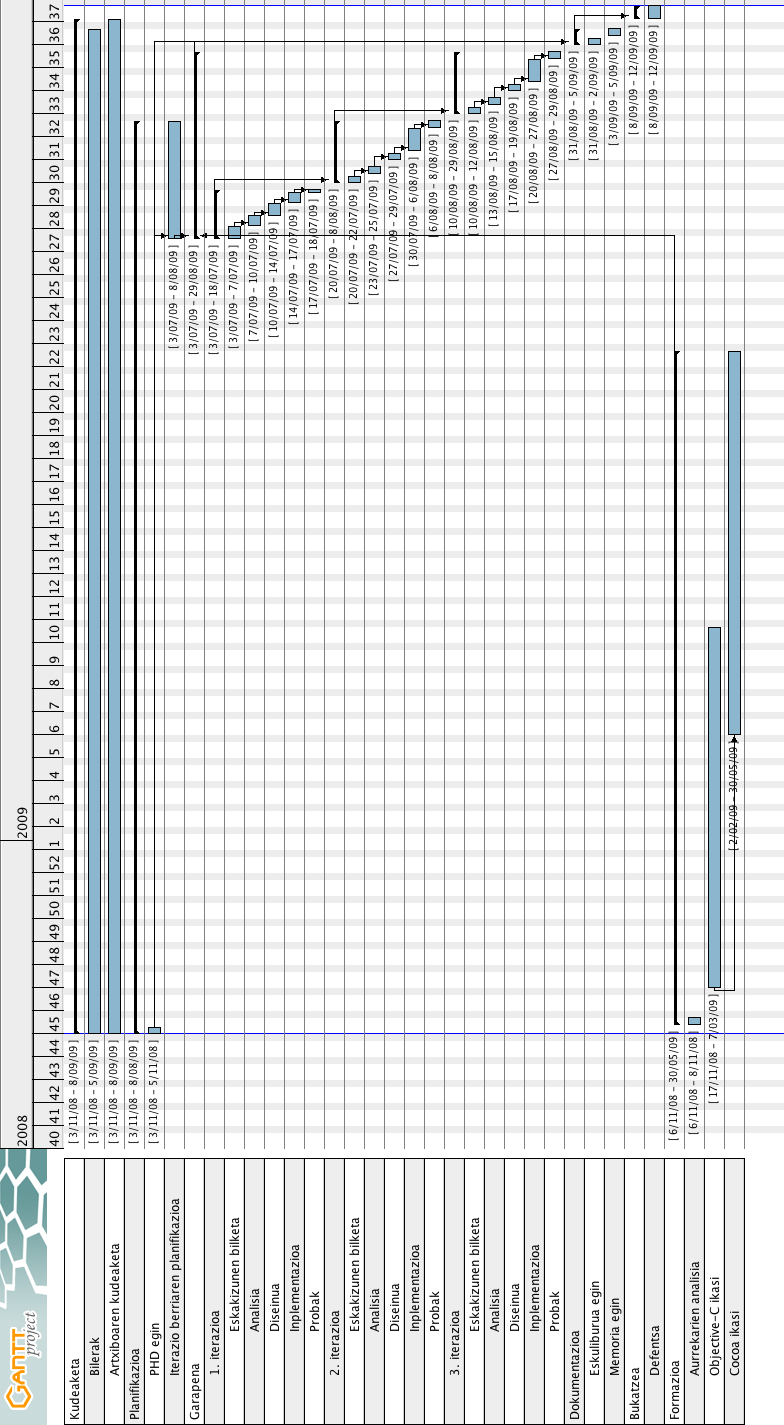
\includegraphics[scale=0.46]{Pictures/Chapter3/Gantt.png}
\caption{Gantt diagrama}
\label{gantt}
\end{center}
\end{figure}

\section{Arriskuak}
Proiektu guztietan kontuan hartu beharreko arriskuan agertzen dira, batzuk beste batzuk baino larriagoak eta gertatzeko probabilitate handiago edo txikiagokoak. Hauek dira aurreikusten diren arriskuak eta gertatzekotan zer egin behar den:
\begin{enumerate}
\item \textit{Atzerapenak proiektuan zehar:}\\
Proiektua garatzen den bitartean, ikaslea SIIT-eko 3. maila egiten egongo da, beraz bi ekintzak aldi berean egingo ditu. Honez gain, bere bizitza pertsonaleko beste aktibitate batzuk ere egingo ditu bitartean.\\
\textbf{Probabilitatea:} altua.\\
\textbf{Ondorioak:} planifikatutako emangarrien atzerapenak.\\
\textbf{Konponbidea:} datak birplanifikatu eta lan erritmoa igo ahal den einean.

\item \textit{Ikasle edo irakaslearen baja gaixotasunagatik:}\\
Ikaslea gaixotzen bada, ezin izango du proiektuan lan egin. Irakaslea aldiz gaixotzen bada, ezin izango du ikaslea gidatu proiektuan zehar.\\
\textbf{Probabilitatea:} baxua.\\
\textbf{Ondorioak:} planifikatutako emangarrien atzerapenak.\\
\textbf{Konponbidea:} esfortzua birplanifikatu entregatze datak betetzeko.

\item \textit{Lan egiteko zerbitzaria atzigarri ez egotea:}\\
Assembla.com erabiliko da garapenean zehar honen tresnak erabiliz, adibidez SVN zerbitzaria han egongo da. Software edo hardware arazoak direla eta agian ezin izango da atzitu denbora tarte batean.\\
\textbf{Probabilitatea:} baxua.\\
\textbf{Ondorioak:} egindako lanaren galera eta lana ezin egitea.\\
\textbf{Konponbidea:} aurretik sortutako babes kopiak erabiltzea.
\end{enumerate}

\section{Lan metodologia}
Proiektu honetan zehar jarraituko den metodologia softwarearen garapenerako prozesu bateratuak (\textbf{SGPB}) definitzen duena izango da. Modelatzeko lengoaia bezala \textit{Unified Modeling Language} (UML) erabiliko da.
\subsection{Bilerak}
Bilerak astean behin edo bi astero egingo dira, lan zamaren menpe. Bilera hauetan ikaslea eta proiektuaren zuzendaria egongo dira. Bertan egindako berrikusiko da planifikatutakoarekin bat datorren ikusteko eta hurrengo bileraren data esleituko da. Honez gain, denbora tarte horretan zein ataza egingo diren planifikatutko da.
\subsection{Teknologiak / Softwarea}
Proiektu honen garapenerako teknologia eta software hauek erabiliko ditugu:
\begin{itemize}
\item \textbf{\LaTeX{}:} dokumentazioa sortzeko markaketa lengoaia. WYSIWYM\footnote{\textit{What You See Is What You Mean} - Ikusten duzuna da egin nahi duzuna. \url{http://en.wikipedia.org/wiki/WYSIWYM}} motakoa da eta dokumentazioa teknikoa sortzeko oso erabilia da. Lana erraztearren, \textbf{itsas}\footnote{\url{http://itsas.ehu.es/}} taldeak eskaintzen duen txantiloia erabiliko da, bertan memoriak eduki behar duen formatua oso ondo definituta dagoelako eta lan asko aurreratuko digulako.

\LaTeX{} lengoaia da soilik, beraz editore bat eta konpiladore bat (iturburu fitxategietatik PDF fitxategi bat lortzeko) beharko ditugu. Editore bezala \textbf{MacVim}\footnote{\url{http://code.google.com/p/macvim}} erabiliko da, Mac OS X-erako vim editore famatuaren bertsio bat. Konpilatzeko \textbf{Mac\TeX}\footnote{\url{http://www.tug.org/mactex/}} distribuzioa erabiliko da, bertan beharko ditugun tresna eta plugin guztiak aurkituko ditugulako.
\item \textbf{iWork:} ofimatikarako suite bat. Nahiz eta \LaTeX{} erabili dokumentazioa sortzeko, behar bada erabili behar izango dugu, adibidez grafikoak sortzeko.
\item \textbf{Dia:} diagramak sortzeko tresna. Gure kasuan UML erabiliko dugunez zenbait diagrama sortu beharko ditugu proiektuan zehar: LDE, EKE, sekuentzia diagramak, klase diagramak, etab.
\item \textbf{GanttProject:} Gantt diagrama sortzeko erabiliko dugu, hau da, proiektuaren ataza desberdinen iraupena deskribatzeko.
\item \textbf{Objective-C 2.0:} objektuei zuzendutako programazio lengoaia, C lengoaiaren gainean eratua. Mac OS X sisteman aplikazioak garatzeko programazio lengoaia erabiliena da. Konpilatzeko ez dugu ezer berezirik behar, \textbf{gcc} konpiladore famatua erabili daitekeelako.

2.0 bertsioan asko lagunduko diguten funtzionalitateak aurkituko ditugu: zabor bilketa, propietateak, \textit{fast enumeration}, etab.
\item \textbf{Cocoa:} objektuei zuzendutako API\footnote{Application Programming Interface} natiboa Mac OS X sistemarako. Objective-C lengoaia erabiltzen du eta sistemarekin bikain integratzen dira API hau erabiltzen duten aplikazioak.
\item \textbf{Xcode:} aplikazioa garatzeko IDE\footnote{Integrated Development Environment}-a. Beste IDE gehienetan aurkitu ditzakegun funtzionalitateak dauzka (araztailea, sintaxi koloreztailea, etab.).
\item \textbf{Interface Builder:} Cocoa aplikazioen interfaze grafikoak eratzeko eta kodearekin \textit{lotzeko} aplikazioa. Bi aplikazio hauek eta gcc konpiladorea Apple-ek eskaintzen ditu dohain: \url{http://developer.apple.com/Tools/}.
\end{itemize} 
\section{Bideragarritasuna}
Ekonomikoki proiektua bideragarria da, ez dugulako dirurik inbertitu behar, garapenerako ekipoak baditugulako. Sistema eragilea kenduta, erabiliko diren tresna eta teknologia guztiak dohainekoak dira, eta horietako batzuk gainera askeak dira.

% TODO: feo feo
Ikuspegi teknologikoa kontuan hartuta ere bideragarria da, egin nahi duguna inplementatuta dagoelako beste sistema eragile batzuetan.

Azkenik, denboraren ikus puntutik, kurtsoan zehar egitea ezinezkoa izango da, ikasleak duen lan zamagatik, beraz, proiektuaren zati handiena udan egin behar izango da, ekaineko azterketak bukatu ondoren. Plangintzaren arabera iraileko bigarren asterako prest egon beharko da.